\documentclass[11pt, oneside]{article} 
\usepackage{geometry}
\geometry{letterpaper} 
\usepackage{graphicx}
	
\usepackage{amssymb}
\usepackage{amsmath}
\usepackage{parskip}
\usepackage{color}
\usepackage{hyperref}

\graphicspath{{/Users/telliott/Github/calculus_book/png/}}
% \begin{center} \includegraphics [scale=0.4] {gauss3.png} \end{center}

\title{Fibonacci numbers}
\date{}

\begin{document}
\maketitle
\Large

\label{sec:fibonacci}

Continuing with the topic of induction, let's introduce the Fibonacci numbers and Binet's formula.  

These are numbers in a series formed by adding together the two previous numbers in the series:
\[ F_n = F_{n-2} + F_{n-1} \]
or
\[ F_{n+1} = F_{n-1} + F_{n} \]

It remains to choose the first two numbers, which are $1$ and $1$.  Thus the first ten Fibonacci numbers are
\[ 1 \ \  1 \ \   2 \ \   3  \ \  5  \ \  8 \ \   13 \ \   21 \ \   34 \ \   55 \]

\subsection*{Fibonacci example}

We will use induction to prove that the sum of the first $n$ Fibonacci numbers is
\[ 1 + 1 + 2 + \dots + F_n = F_{n+2} - 1 \]
We assume that the formula is correct for $F_{n - 1}$:
\[ 1 + 1 + 2 + \dots + F_{n-1} = F_{n+1} - 1 \]
Add $F_{n}$ to both sides
\[ 1 + 1 + 2 + \dots + F_{n} = F_{n} + F_{n+1} - 1 \]
\[ = F_{n+2} - 1 \]

This completes the induction.

The base case is 
\[ 1 = 2 - 1 \]

$\square$

Another way to check this is to write the sum as

\begin{verbatim}
 1 + 1 + 2 + 3 + 5 + ..      .. + F_{n}   + F_{n+1}
     1 + 1 + 2 + 3 + 5 + ..  .. + F_{n-1} + F_{n}
 --------------------------------------------------
 1 + 0 + 1 + 1 + 2 + ..      .. + F_{n-2} + F_{n-1}
\end{verbatim}

Subtracting the second sum from the first, we obtain the third:
\[ \sum F_{n+1} - \sum F_n =  \sum F_{n-1} + 1  \]
\[ F_{n+1}  =  \sum F_{n-1} + 1  \]
which rearranges to give the formula.

\subsection*{Binet}

Binet's formula is an explicit formula for $F_n$ which saves us from calculating all the intermediate numbers:
\[ F_n = \frac{\phi^n - \psi^n}{\phi - \psi} \]
where $\phi$ is the Golden Ratio $(1 + \sqrt{5})/2$ and $\psi$ is its conjugate $(1 - \sqrt{5})/2$.

\subsection*{Golden ratio}
The basic definition involves the following construction:
\begin{center} 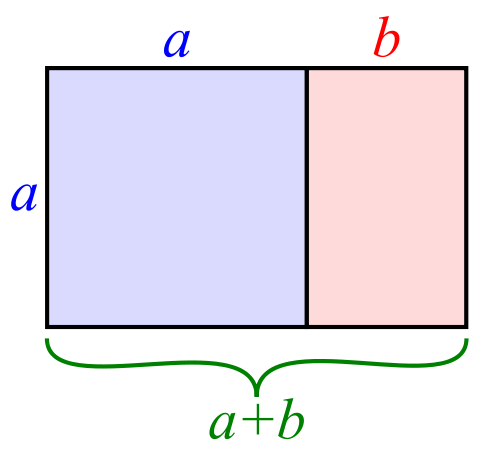
\includegraphics [scale=0.3] {goldenratioab.png} \end{center}
We start with a square of side length $a$ and then extend one side by length $b$, forming two rectangles.  When the ratios of side lengths for these two rectangles are the same, then that ratio is the golden ratio:
\[ \phi = \frac{a}{b} = \frac{a + b}{a} \]
($\phi$ is often written $\Phi$).

Rescaling of the figure in both dimensions doesn't change the ratios, so let $b = 1$.  Then (changing to the symbol $\phi$):
\begin{center} 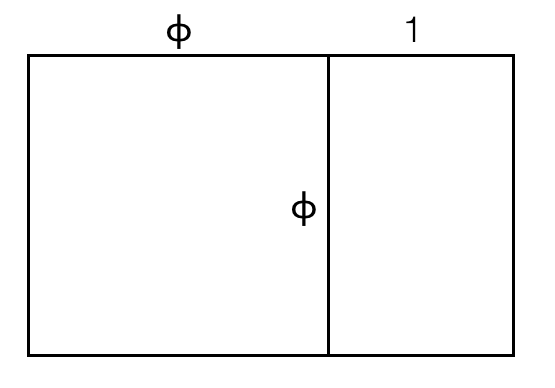
\includegraphics [scale=0.3] {phi.png} \end{center}
\[ \frac{\phi}{1} = \frac{\phi + 1}{\phi} \]
\[ \phi^2 = 1 + \phi \]
We will need only this last result below.  

The equation can be solved numerically using the quadratic formula.  Put everything on the left-hand side
\[ \phi^2 - \phi - 1 = 0 \]
Recall that the solutions are
\[ \frac{-b \pm \ \sqrt{b^2 - 4ac}}{2a} \]
We obtain
\[ \phi = \frac{1 + \sqrt{5}}{2} \ \ \ \  \psi = \frac{1 - \sqrt{5}}{2} \]
This gives values of $\phi \approx 1.61803$ and $\psi \approx - 0.61803$.  

It seems like $\phi = 1 - \psi$.  Proof:
\[ 2 \phi = 1 + \sqrt{5} \]
\[ 2 \psi = 1 - \sqrt{5} \]
Adding them together
\[ 2(\phi + \psi) = 2 \]
What a nice symmetry:
\[ \phi + \psi = 1 \]
\[ \phi = 1 - \psi \]
\[ \psi = 1 - \phi \]

Note that since $\psi$ is a solution it is also true that
\[ \psi^2 = 1 + \psi \]
An alternative proof of that is:
\[ \psi^2 = (1 - \phi)^2 \]
\[ = 1 - 2 \phi + \phi^2 \]
\[ = 1 - 2\phi + 1 + \phi \]
\[ = 2 - \phi = 2 - (1 - \psi) = 1 + \psi  \]

We can also do the arithmetic
\[ \phi^2 = \frac{1 + \sqrt{5}}{2} \cdot \frac{1 + \sqrt{5}}{2} = \frac{6 + 2 \sqrt{5}}{4} = 1 + \phi \]
\[ \psi^2 = \frac{1 - \sqrt{5}}{2} \cdot \frac{1 - \sqrt{5}}{2} = \frac{6 - 2 \sqrt{5}}{4} = 1 + \psi \]

\subsection*{back to the proof}
Wikipedia says that you can prove Binet's formula using induction.
\[ F_n = \frac{\phi^n - \psi^n}{\phi - \psi} \]

\url{https://en.wikipedia.org/wiki/Mathematical_induction#Example:_Fibonacci_numbers}

That is an entertaining challenge.  For induction we assume that the formula is correct for $F_{n-1}$ and $F_n$ and must prove that:
\[ F_{n+1} = F_n + F_{n-1} \]
\[ = \frac{\phi^n - \psi^n}{\phi - \psi} + \frac{\phi^{n-1} - \psi^{n-1}}{\phi - \psi} \]
\[ = \frac{(\phi^n + \phi^{n-1}) - (\psi^{n} + \psi^{n-1})}{\phi - \psi} \]

Although one could imagine it is more complicated, the simple idea is to try to show that
\[ \phi^{n+1} = \phi^n + \phi^{n-1} \]
and the same for $\psi$, and that will complete the proof of the inductive step.

Write
\[ \phi^{n+1} = \phi^2 \ \phi^{n - 1} = (1 + \phi) \ \phi^{n - 1} = \phi^{n-1} + \phi^n  \]
similarly
\[ \psi^{n+1} = \psi^2 \ \psi^{n - 1} = (1 + \psi)\psi^{n-1} = \psi^{n-1} + \psi^n \]
This shows that the inductive step is valid.

Now we just need to verify the base cases.  We should check at least the first two of them, because there are two values in the recursion formula $F_{n} + F_{n-1}$.

It's a matter of convenience whether we consider the series to start with $n=1$ or $n=0$.  If the latter, then the zeroth Fibonacci number is $0$, and the first is $1$ and we obtain the same series.

For $n = 0$ we have $\phi^0 - \psi^0$ which is just zero.

For $n = 1$, we have 
\[ \frac{\phi^1 - \psi^1}{\phi - \psi}  = 1 \]

We decide to continue with $n = 2$
\[ \phi^2 = \phi + 1 \]
\[ \psi^2 = \psi + 1 \]
so
\[ \frac{\phi^2 - \psi^2}{\phi - \psi} = \frac{\phi + 1 - \psi - 1}{\phi - \psi} = 1 \]
This completes the proof. 

$\square$

At this point we note the curious pattern
\[ \phi^2 = \phi + 1 \]
\[ \phi^3 = \phi^2 + \phi = 2 \phi + 1 \]
\[ \phi^4 = \phi^2 + 2 \phi + 1 = 3 \phi + 2 \]
\[ \phi^5 = 2 \phi^2 + 3 \phi + 1 =  5 \phi + 3 \] 
\[ \phi^6 = 4 \phi^2 + 4 \phi + 1 = 8 \phi + 5 \]
so it looks like
\[ \phi^n = F_n \ \phi + F_{n-1} \]

The coefficients \emph{are} the Fibonacci numbers.  

The same is true for $\psi$ since $\psi^2 = \psi + 1$.

We could prove this by induction, and it would be a proof of Binet's formula as well because the coefficient of $\phi^n$ or $\psi^n$ is equal to $F_n$ so
\[ \phi^n = F_n \ \phi + F_{n-1} \]
\[ \psi^n = F_n \ \psi + F_{n-1} \]
and then
\[ \frac{\phi^n - \psi^n}{\phi - \psi} = \frac{(F_n \ \phi + F_{n-1}) - (F_n \ \psi + F_{n-1})}{\phi - \psi} \]
\[ = F_n \ \frac{\phi - \psi}{\phi - \psi}  = F_n \]


\end{document}